\documentclass[10pt,letterpaper]{article}
\newcommand{\tab}[1]{\hspace{.1\textwidth}\rlap{#1}}
\usepackage{calc}
\usepackage{fullpage}
\usepackage{pgfplots}
\pgfplotsset{compat=1.12}
\usepackage{graphicx}
\graphicspath{ {images/} }

\begin{document}
	\title{Math 360 Project 2: Allometry}
	\author{Erica Chase}
	\date {October 2, 2015}
	\maketitle
	\section{Introduction}
		In biology, allometry is defined as the change in proportion of any of the parts of an organism that occurs during growth. For example, in humans, breathing and heart rate ($t$) are both proportional to body mass ($M$) raised to the $\frac 1 4$ power: $t \propto M^{\frac 1 4}$. In general, allometric models tend to follow power law functions, such as $x = ky^{a}$, where $x$ is the quantity of interest, $k$ is a constant of proportionality, $y$ is some measure of size, and $a$ is a constant exponent. Many factors can play into allometry, such as environment and resources, physiological and mechanical design design, and generational evolutionary changes. 
	\section{Parameters}
		\begin{center}
			\begin{tabular}{c l}
				Parameter & Definition \\
				\hline \hline
				$x$ & Quantity of Interest \\
				$k$ & Proportionality constant \\
				$y$ & Measure of size \\
				$a$ & Constant exponent \\
				\hline
				$R_{D}$ & Reproductive desirablity \\
				$C$ & Claw size \\
				$b$ & Exponential constant for mass \\
				\hline
				$B$ & Basal metabolic rate \\
				$M$ & Mass \\
				\hline
				$S$ & Brain size
			\end{tabular}
		\end{center}
	\section{Fiddler Crab}
		The male fiddler crap is a perfect exmple of allometry; they have an enlarged major claw, used for fighting and threatening other males and attracting females, that is proportional to their $mass^{b}$. Additionally, their reproductive desireability ($R_{D}$) is proportional to their claw size ($C$). This can be displayed as:
		\newline \newline
		\centerline{$R_{D} \propto C \propto mass^{b}$}
		\newline \newline
		Given this information, we can combine it with standard allometric power law functions to obtain a model. We know that the standard power law function format follows $x = ky^{a}$ and that $R_{D} \propto C \propto mass^{b}$, meaning $R_{D} \propto mass^{b}$. Since reproductive desirability is the quantity of interest, we can replace $x$ with $R_{D}$. Additionally, we know that size is being measured as mass, raised to the power of $b$. Thus, we can subsitute $y^{a}$ with $mass^{b}$. Finally, we need a proportionality constant, which we will leave as $k$. this gives a new model to measure reproductive disirability as a function of mass:
		\newline \newline
		\centerline{$R_{D} = k (mass)^{b}$}
		\subsection{Logarithmic Transformation and Linear Regression}
			In the problem, we're given data for the mass and claw mass of 10 fiddler crabs:
			\begin{center}
				\begin{tabular}{c c}
					Mass (g) & Claw mass (g)\\
					\hline
					4.74516 & 0.303208 \\
					10.4439 & 1.15915 \\
					14.1628 & 1.24838 \\
					18.8073 & 1.65723 \\
					23.2829 & 2.65709 \\
					29.0201 & 3.14769 \\
					33.2396 & 2.82348 \\
					37.577  & 5.27659 \\
					42.7777 & 7.44482 \\
					49.6655 & 5.50366
				\end{tabular}
			\end{center}
			The scatter plot for this data looks like this:
			\newline \newline
			\centerline{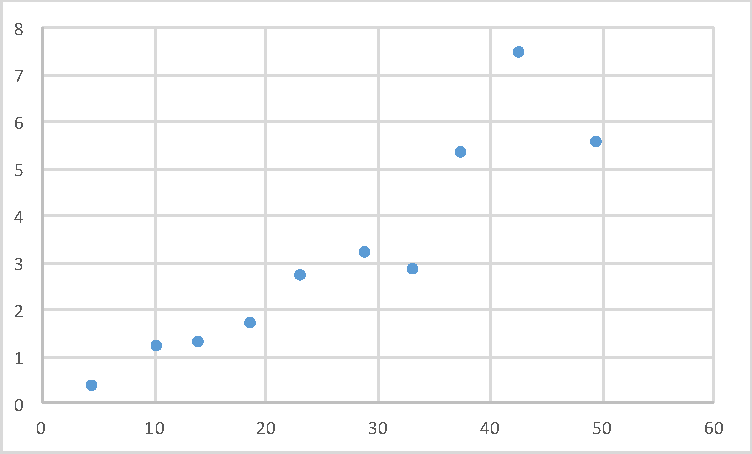
\includegraphics{Picture1.pdf}}
			\newline \newline
			As can be seen, this data has a very wide range that makes it difficult to fit a model to. Fortunately, we're able to use logarithmic transformations to rescale the data into something that's much easier to work with. The new data looks like this:
			\begin{center}
				\begin{tabular}{c c}
					ln(Mass) (g) & ln(Claw mass) (g)\\
					\hline
					1.55713 & -1.19334 \\
					2.34602 & 0.147687 \\
					2.65062 & 0.221847 \\
					2.93425 & 0.505148 \\
					3.14772 & 0.977232 \\
					3.367989 & 1.14667 \\
					3.503742 & 1.03797 \\
					3.62639 & 1.66328 \\
					3.756017 & 2.00752 \\
					3.905311 & 1.70541
				\end{tabular}
			\end{center}
			This transformation scales the data so that the mass only ranges from about 1g to 4g and the claw mass ranges from roughly 0g to 2g. An interesting outlier to note the the claw mass value of -1.9334g when the crab weighs 1.55713g. The claw mass value cannot be negative, so the logarithmic transformation can only work for a certain range of values. That scatter plot for the transformed data looks like this:
			\newline \newline
			\centerline{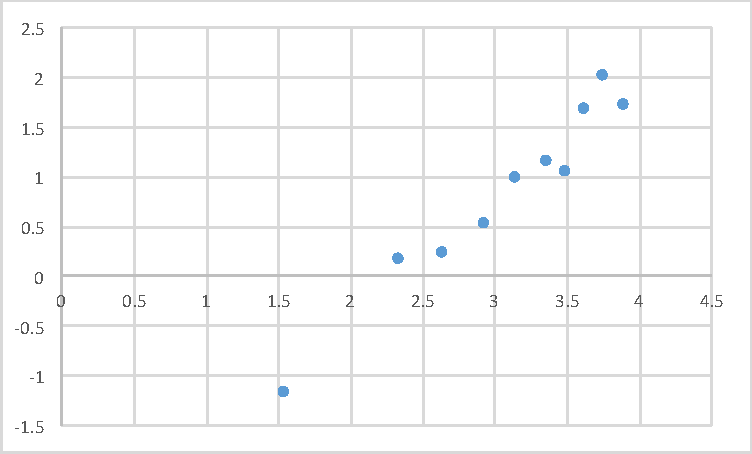
\includegraphics{Picture2.pdf}}
			\newline \newline
			This plot visibly looks much more linear, making it much easier to model via linear regression. 
		\subsection{Model Fit}
			Using a linear fit, we can derive a new plot:
			\newline \newline
			\centerline{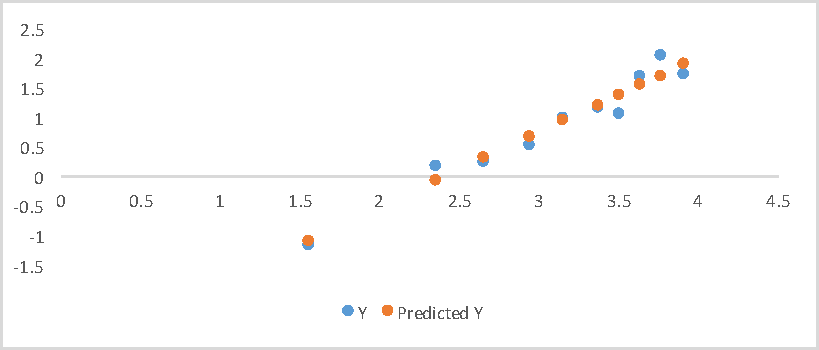
\includegraphics{Picture3.pdf}}
			\newline \newline
			The resulting linear model is $C = 1.2698(mass) - 3.0886$. There is also a set of data displaying the original transformed data vs. the data from the regression fit, as well as the error between the two:
			\begin{center}
				\begin{tabular}{c c c}
					ln(Mass) (g) & ln(Mass) (g) [fit] & Error \\
					\hline
					-1.19334 & -1.111250159 & -0.082089841 \\
					0.147687 & -0.109484922 & 0.257171922 \\
					0.221847 & 0.27730879 & -0.05546179 \\
					0.505148 & 0.637473926 & -0.132325926 \\
					0.977232 & 0.908546985 & 0.068685015 \\
					1.14667 & 1.188253696 & -0.041583696 \\
					1.03797 & 1.360638485 & -0.322668485 \\
					1.66328 & 1.516382002 & 0.146897998 \\
					2.00752 & 1.680987742 & 0.326532258 \\
					1.70541 & 1.870567454 & -0.165157454
				\end{tabular}
			\end{center}
			The relatively small values for the error indicate that the new model is very very close to the original data. However, we can also skip the original logarithmic transformation to apply a curve fit to the first set of data. Loosely, the original scatter plot appears visually like an exponential function, where $C = .001 \times (mass)^{2}$. Using this, we can modify the exponential function to beter fit our data, such as:
		\subsection{Model Extrema}
	\section{Metabolism}
	% Kleiber's law, metabolic rate q_{0} is proportional to body mass M raised to the 3/4 power:
	% q_{0} \sim M^{\frac 3 4}
		Another important allometric relationship is that of metabolism to surface area. Specifically, the amount of heat energy an animal produces is proportional to the amount of surface area required to radiate or absorb heat. However, it's very difficult to accurately measure the surface area of most animals, so a model that depends on mass is very helpful. 
		\subsection{Power Law Model}
			One important law to note is Kleiber's law, which states that an animal's metabolic rate is proportional to its body mass raised to the $\frac 3 4$ power or $B \propto M^{\frac 3 4}$. Using a proportionality constant, $k$, we can derive a model, such that $B = kM^{\frac 3 4}$.
		\subsection{Regression and Outliers}
			The problem gives us a set of data that relates the body mass of a certain number of species to their basal metabolic rate, seen below:
			\begin{center}
				\begin{tabular}{l c c}
					Species & Mass (g) & BMR (kJ/h) \\
					\hline
					\emph{Geogale aurita} & 6.9 & 0.16 \\
					\emph{Dromiciops gliroides} & 40 & 0.64 \\
					\emph{Tupaia glis} & 123 & 1.88 \\
					\emph{Caluromys debaianus} & 357 & 4.09 \\
					\emph{Isoodon auratus} & 428 & 3.01 \\
					\emph{Philander opossum} & 751 & 6.79 \\
					\emph{Macrotis lagotis} & 1011 & 7.11 \\
					\emph{Aotus trivirgatus} & 1020 & 9.22 \\
					\emph{Tachyglossus aculeatus} & 2140 & 5.63 \\
					\emph{Propithecus verrauxi} & 3080 & 13.73 \\
					\emph{Didelphis virginana} & 3257 & 21.58 \\
					\emph{Macropus eugenii} & 4796 & 27.93 \\
					\emph{Ailurus fulgens} & 5740 & 17.64 \\
					\emph{Zaglossus bartoni} & 10300 & 24.41 \\
					\emph{Lasiorhunus latifrons} & 25000 & 50.2 \\
					\emph{Phocoena phocoena} & 28500 & 389.00 \\
					\emph{Pan troglodytes} & 33900 & 182.43 \\
					\emph{Orycteropus afer} & 48000 & 123.37 \\
					\emph{Homo sapiens} & 60500 & 255.12 \\
					\emph{Panthera tigris} & 137900 & 481.81 \\
					\emph{Tursiops truncates} & 148600 & 1163.72 \\
					\emph{Ursus arctos} & 170000 & 395.99 \\
					\emph{Alces americanus} & 350000 & 11455.6 \\
					\emph{Leptonychotes weddelli} & 388500 & 1497.81 \\
					\emph{Orcinus orca} & 3221000 & 7826
				\end{tabular}
			\end{center}
			Once again, the wide range of this data makes it very difficult to plot in a meaningful way. Espcially with the inclusion of the \emph{Orcinus orca}, the current plot is very difficult to read:
			\newline \newline
			\centerline{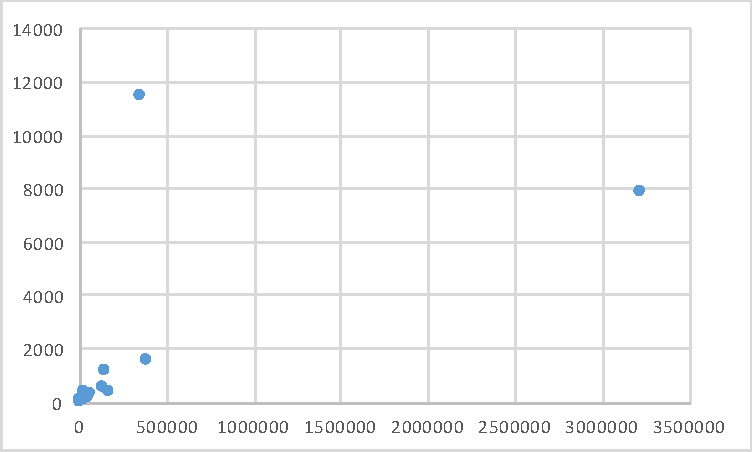
\includegraphics{Picture7.pdf}}
			\newline \newline 
			Using a logarithmic transformation, we obtain this new set of data:
			\begin{center}
				\begin{tabular}{l c c}
					Species & log(Mass) (g) & log(BMR) (kJ/h) \\
					\hline
					\emph{Geogale aurita} & 0.838849091 & -0.795880017 \\
					\emph{Dromiciops gliroides} & 1.602059991 & -0.193820026 \\
					\emph{Tupaia glis} & 2.089905111 & 0.274157849 \\
					\emph{Caluromys debaianus} & 2.552668216 & 0.611723308 \\
					\emph{Isoodon auratus} & 2.631443769 & 0.478566496 \\
					\emph{Philander opossum} & 2.875639937 & 0.831869774 \\
					\emph{Macrotis lagotis} & 3.004751156 & 0.851869601 \\
					\emph{Aotus trivirgatus} & 3.008600172 & 0.964730921 \\
					\emph{Tachyglossus aculeatus} & 3.330413773 & 0.750508395 \\
					\emph{Propithecus verrauxi} & 3.488550717 & 1.137670537 \\
					\emph{Didelphis virginana}  & 3.512817759 & 1.33405144 \\
					\emph{Macropus eugenii} & 3.680879174 & 1.446070936 \\
					\emph{Ailurus fulgens} & 3.758911892 & 1.246498581 \\
					\emph{Zaglossus bartoni} & 4.012837225 & 1.387567779 \\
					\emph{Lasiorhunus latifrons} & 4.397940009 & 1.700703717 \\
					\emph{Phocoena phocoena} & 4.45484486 & 2.589949601 \\
					\emph{Pan troglodytes} & 4.530199698 & 2.261096258 \\
					\emph{Orycteropus afer} & 4.681241237 & 2.091209565 \\
					\emph{Homo sapiens} & 4.781755375 & 2.406744506 \\
					\emph{Panthera tigris} & 5.139564266 & 2.68287581 \\
					\emph{Tursiops truncates} & 5.172018809 & 3.065848498 \\
					\emph{Ursus arctos} & 5.230448921 & 2.597684219 \\
					\emph{Alces americanus} & 5.544068044 & 4.059017841 \\
					\emph{Leptonychotes weddelli} & 5.589391023 & 3.175456726 \\
					\emph{Orcinus orca} & 6.507990725 & 3.893539844 
				\end{tabular}
			\end{center}
			Plotting this data gives us a much more linear visual of the data, making it easier to fit a new model.
			\newline \newline
			\centerline{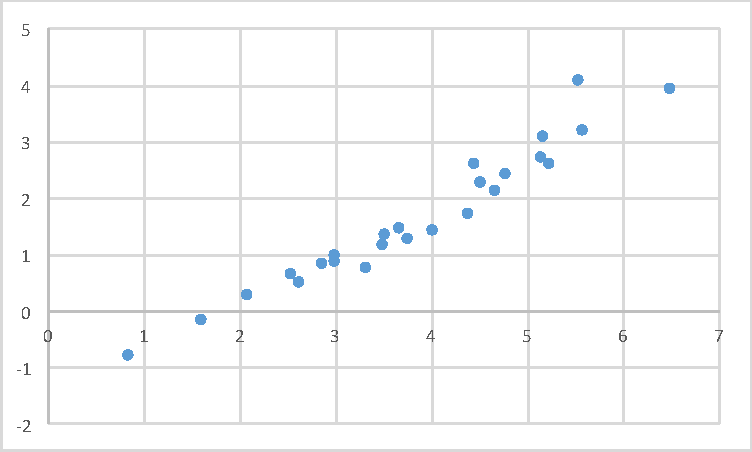
\includegraphics{Picture8.pdf}}
			\newline \newline
			Using a linear regression, we obtain a linear model of $B = 0.876722M - 1.74727$. We can plot both the linear fit and the original transformation on the same graph to see the similarities between the two:
			\newline \newline
			\centerline{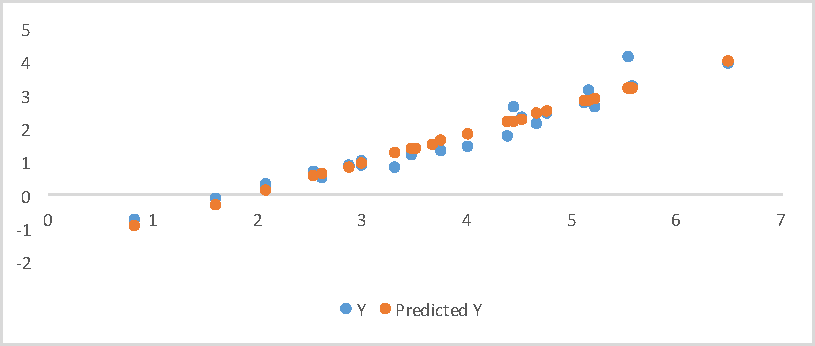
\includegraphics{Picture9.pdf}}
			\newline \newline
			While there are a couple obvious outliers, generally the regression seems to be a very good fit. One major outlier is the \emph{Alces americanus}, or moose. The moose's basal metabolic rate is oddly close to is mass, especially in the logarithmic transformation. Removing this data point does not significantly change the regression, but does create a new fit where $B = 0.836507M - 1.63441$.
		\subsection{Non-linear Regression}
		\subsection{Further Exploration}
			Another interesting example of biological allometry is shown in “Brain Size, Life History, and Metabolism at the Marsupial/placental Dichotomy.” by Vera Weisbecker and Anjali Goswami. Specifically, the article observes the relationship between mammallian basal metabolic rate and brain size. Although this correlation is heavily debated, many scientists are beginning to find a relationship between the two. We can use the standardaized allometric power model to derive a model representing the proportionality of brain size ($S$) to basal metabolic rate ($B$), or $S \propto B^{a}$:
			\newline
			\centerline{$S = kB^{a}$}
			\newline
			An important note the article makes is that there are two types of animals that have developed large brains, mammals and birds. These two groups also consistenly have a higher BMR than other animals. This makes sense as it requires much more energy to maintain a larger brain and associated brain function. 
			\newline \newline
			Additionally, the article notes an important correlation between brain size and body mass. Using our above proportionality model, we can observe all three variables together as:
			\newline
			\centerline{$S \propto B^{A} \propto M^{\frac 3 4}$}
			\newline
			For a select group of mammals, the following set of data shows a standardized brain size to body ratiofor each mammal:
			\begin{center}
				\begin{tabular}{l c}
					Species & Brain-to-body ratio \\
					\hline 
					Human & $1/40$ \\
					Mouse & $1/40$ \\
					Dolphin & $1/50$ \\
					Cat & $1/100$ \\
					Chimpanzee & $1/113$ \\
					Dog & $1/125$ \\
					Lion & $1/550$ \\
					Elephant & $1/560$ \\
					Horse & $1/600$ \\
					Hippopotamus & $1/2789$
				\end{tabular}
			\end{center}
			And a visual representation can be seen below:
			\newline \newline
			\centerline{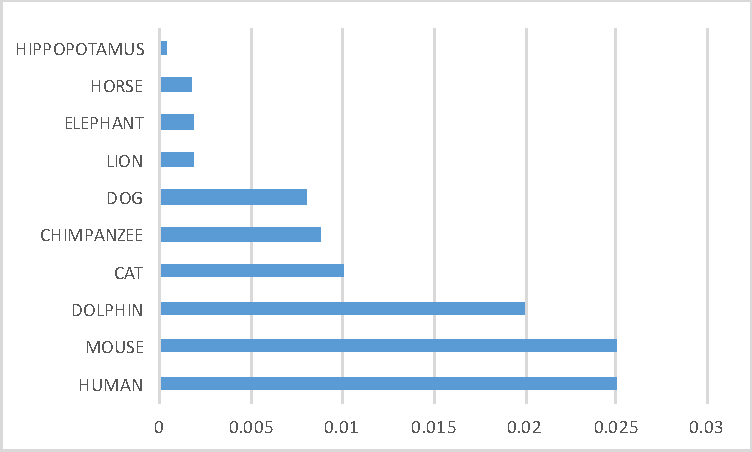
\includegraphics{Picture10.pdf}}
			\newline \newline
			With the exception of humans and dolphins, the data seems to directly show a strong correlation between body mass and brain size; that is, as body mass increases, the brain size grows by a smaller proportion. The smallest mammal, the mouse, has the largest brain size compared to its body, and the larger mammals, such as the elephant or the hippopotamus, have the smallest brains compared to their body mass. This makes sense assuming maintained proportionality with BMR, as more energy is alloted towards running a larger body than a smaller one. The obvious outliers, the human and the dolphin, may be the result of other factors, such as gestational period and postnatal independence. 
	\section{Conclusion}
		
\end{document}

